\section{UML Class Diagram}
\begin{figure}[H]
    \centering
    % Se vuoi riutilizzare la stessa immagine, punta al percorso dell'iterazione precedente
    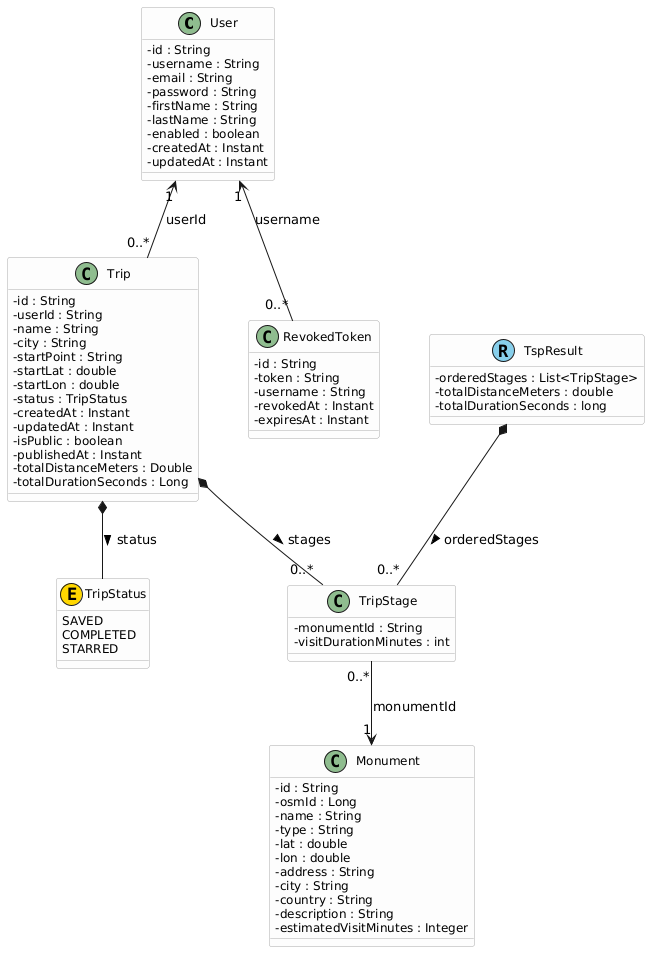
\includegraphics[width=0.9\textwidth]{Iterazione2/Diagrammi/ClassDiagram2.png}
    \caption{UML Class Diagram - Invariato rispetto all'Iterazione 2.}
    \label{fig:class_diagram_it3}
\end{figure}
L'UML Class Diagram per la terza iterazione non ha subito modifiche strutturali rispetto alla versione presentata nell'Iterazione 2. L'architettura delle classi definita precedentemente si è dimostrata sufficientemente flessibile e robusta per supportare l'integrazione delle nuove funzionalità di gestione del profilo utente e della sicurezza (UC2.1 e UC2.2) senza richiedere alterazioni nella gerarchia o nelle relazioni tra le entità principali del sistema.
